\documentclass{beamer}
\usetheme{Warsaw}
\usepackage{lmodern}
\usepackage[french]{babel}
\usepackage[T1]{fontenc}
\usepackage[utf8]{inputenc}
\usepackage{graphicx}

\begin{document}
\title{}
\title{\textbf{Soutenance SIG}}
\author[FONTORBE, FRANÇOIS, MOROSI, PERRIN]{
	\textit{Jordan FONTORBE}\\
	\textit{Willy FRANÇOIS}\\
	\textit{Jérémy MOROSI}\\
	\textit{Jean-Baptiste PERRIN}
}
\maketitle

\tableofcontents

\section{Réalisation}

\subsection{Commun}
\subsubsection{Package data}
\begin{frame}
\frametitle{Package data}

Le modèle :\\
\begin{columns}
\begin{column}{.49\textwidth}
\begin{block}{Bases}
\begin{itemize}
\visible<1->{
\item Node : une latitude et longitude
}
\visible<2->{
\item Road : une liste de noeud, un type (route, chemin, etc.)
}
\end{itemize}
\end{block}
\end{column}
\begin{column}{.49\textwidth}
\visible<3->{
\begin{block}{Structure: nom, liste de noeuds}
\begin{itemize}
\item Building : liste de trous
\item Basin
\item Forest
\item Hole : la structure auquel il appartient
\end{itemize}
\end{block}
}
\end{column}
\end{columns}
\end{frame}

\begin{frame}
\frametitle{Package data}
\begin{block}{Pré-traitement des données}
\begin{itemize}
\item Import des données OSM dans PostgreSQL
\item Récupération des données nécessaires
\item Création de nouvelles tables
\item Création du XML représentant la carte
\end{itemize}
\end{block}
\end{frame}

\begin{frame}
\begin{figure}
\centering
\resizebox{\linewidth}{!}{
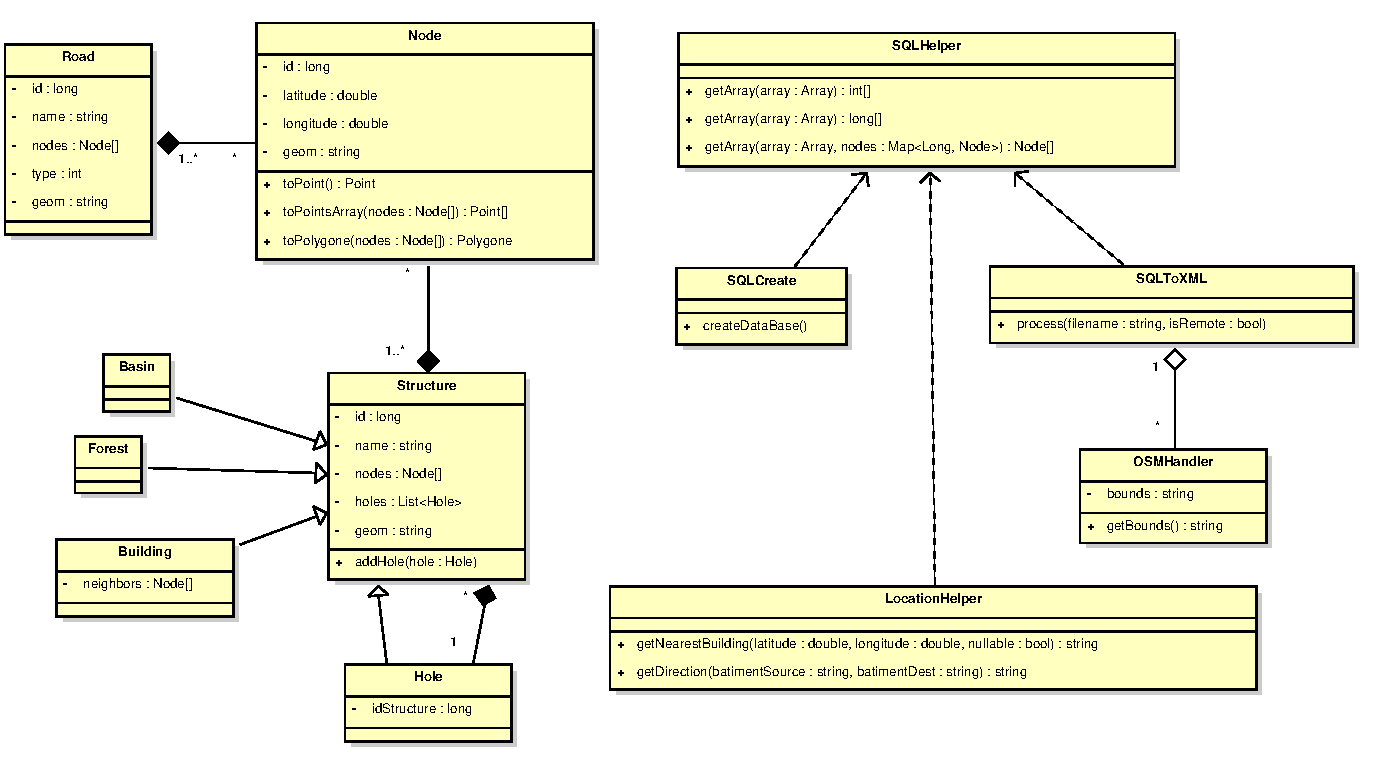
\includegraphics{../images/communData.pdf}
}
\caption{Modèle commun}
\end{figure}
\end{frame}


\subsection{WebService}
\begin{frame}
\frametitle{WebService}
\begin{block}{Méthodes nécessaires pour le mode `remote'}
\begin{itemize}
\item Récupération de la map (format XML)
\item Récupération d'un bâtiment à partir de coordonnées (format JSON)
\item Récupération d'un itinéraire à partir d'un bâtiment de départ et d'arrivée (format JSON)
\end{itemize}
\end{block}
\end{frame}

\begin{frame}
\begin{figure}
\centering
\resizebox{\linewidth}{!}{
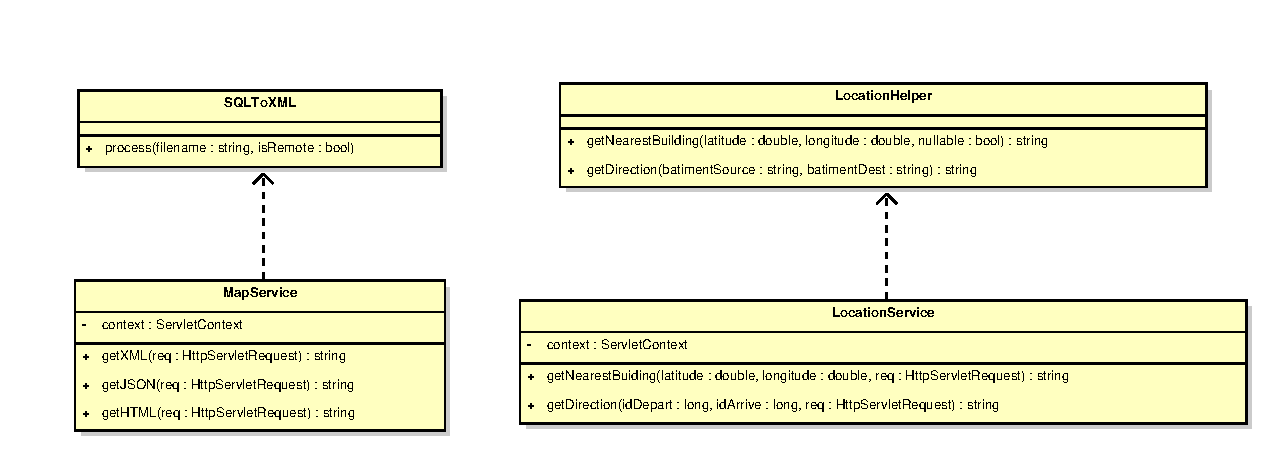
\includegraphics{../images/webService.pdf}
}
\caption{Web Service}
\end{figure}
\end{frame}

\subsection{Android}
\begin{frame}
\frametitle{Android}
\begin{block}{ActivityBase}
\begin{itemize}
\item Affichage de la carte
\item Réception des données du GPS
\item Lien entre l'utilisateur et l'affichage
\end{itemize}
\end{block}
\begin{block}{ISig1337}
\begin{itemize}
\item Méthodes communes pour récupérer:\begin{itemize}
\item Les éléments (bâtiments, routes...)
\item Le bâtiment à partir de coordonnées
\item L'itinéraire entre deux bâtiments
\end{itemize}
\end{itemize}
\end{block}
\end{frame}

\begin{frame}
\frametitle{Android}
\begin{block}{LocalActivity}
\begin{itemize}
\item Utilise LocalSig1337
\end{itemize}
\end{block}
\begin{block}{LocalSig1337}
\begin{itemize}
\item Implémente les méthodes de l'interface en:\begin{itemize}
\item Utilisant l'arbre de décision
\item Utilisant le graphe
\end{itemize}
\end{itemize}
\end{block}
\end{frame}

\begin{frame}
\frametitle{Android}
\begin{block}{RemoteActivity}
\begin{itemize}
\item Utilise RemoteSig1337
\end{itemize}
\end{block}
\begin{block}{RemoteSig1337}
\begin{itemize}
\item Implémente les méthodes de l'interface en:\begin{itemize}
\item Appelant le WebService
\end{itemize}
\end{itemize}
\end{block}
\end{frame}

\begin{frame}
\begin{figure}
\centering
\resizebox{\linewidth}{!}{
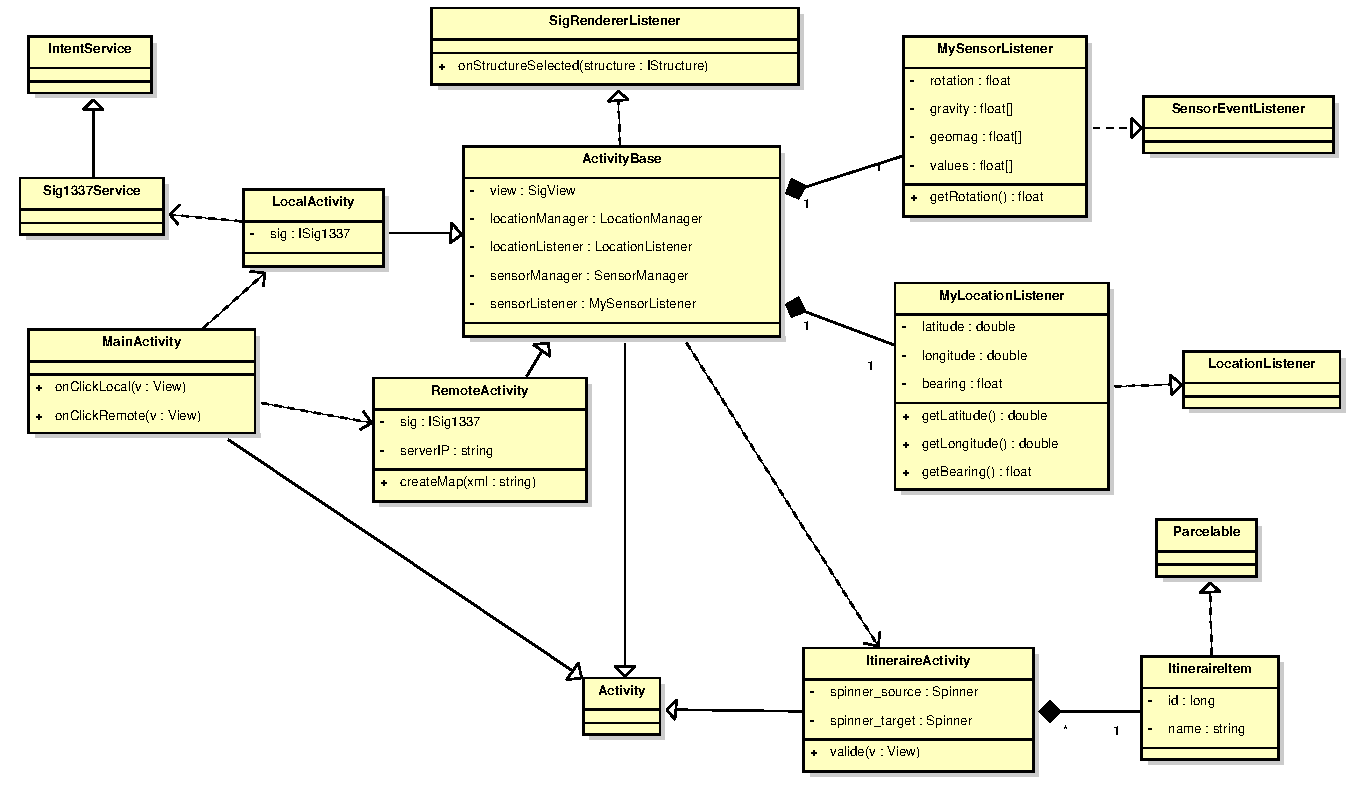
\includegraphics{../images/androidActivity.pdf}
}
\caption{Architecture android}
\end{figure}
\end{frame}


\section{Difficultés rencontrées}
\begin{frame}
\frametitle{Difficultés rencontrées}
\begin{alertblock}{$\underline{/\hat{!}\backslash}$}
\begin{itemize}
\item Import des données OpenStreetMap
\item Arbre de décision
\item Itinéraire en local
\end{itemize}
\end{alertblock}
\end{frame}


\section{Conclusion}
\begin{frame}
\end{frame}


\end{document}
